\documentclass{article}
\usepackage[utf8]{inputenc}
\usepackage{graphicx}
\usepackage{listings}
\usepackage{xcolor}
\usepackage{hyperref}
\usepackage{geometry}
\usepackage{float}
\geometry{margin=1in}

\lstset{ %
  language=Java,
  basicstyle=\ttfamily\small,
  numbers=left,
  numberstyle=\tiny,
  stepnumber=1,
  numbersep=5pt,
  backgroundcolor=\color{white},
  showspaces=false,
  showstringspaces=false,
  showtabs=false,
  frame=single,
  tabsize=2,
  captionpos=b,
  breaklines=true,
  breakatwhitespace=false,
  keywordstyle=\color{blue},
  commentstyle=\color{green!50!black},
  stringstyle=\color{orange},
  morecomment=[l]{//},
  morecomment=[s]{/*}{*/},
  numberblanklines=false,
  caption={\empty}, % Removes the "Listing" numbering
  label={}, % Clears the label reference
  literate=
    % Replacements for special characters
    {~}{{\textasciitilde}}1
    {\#}{{\#}}1
    {\$}{{\$}}1
    {\%}{{\%}}1
    {\&}{{\&}}1
    {\_}{{\_}}1
    {\{}{{\{}}1
    {\}}{{\}}}1
    {^}{{\^{}}}1
    {<}{{\textless}}1
    {>}{{\textgreater}}1
}

\renewcommand{\lstlistingname}{} % removes "Listing" label

\begin{document}

\section*{Assignment 1}

\subsection*{Problem 1}

\begin{figure}[H]
    \centering
    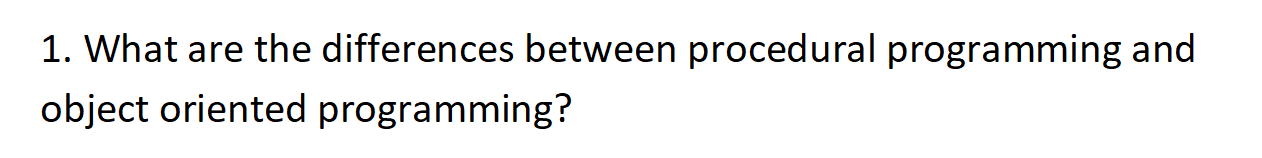
\includegraphics[width=0.8\textwidth]{./Assets/Task requirements/Assignment1/1.png}
    \caption{Problem 1 Task Requirement}
\end{figure}

\textbf{Core Concepts}
\begin{itemize}
    \item \textbf{Procedural Programming}: Focuses on functions and procedures to execute a sequence of tasks.
    \item \textbf{OOP}: Centers on objects, which encapsulate data and behaviors (methods).
\end{itemize}

\textbf{Structure}
\begin{itemize}
    \item \textbf{Procedural}: Organized in a linear flow of functions.
    \item \textbf{OOP}: Organized around classes and objects.
\end{itemize}

\textbf{Data Handling}
\begin{itemize}
    \item \textbf{Procedural}: Data and functions are separate; data is passed to functions.
    \item \textbf{OOP}: Data and functions are bundled; methods operate on object data.
\end{itemize}

\textbf{Key Features}
\begin{itemize}
    \item \textbf{Encapsulation}: OOP promotes data hiding and access control; procedural programming has minimal encapsulation.
    \item \textbf{Inheritance}: OOP supports inheritance for code reuse; procedural does not.
    \item \textbf{Polymorphism}: OOP allows method overloading and overriding; procedural has limited support.
\end{itemize}

\textbf{Use Cases}
\begin{itemize}
    \item \textbf{Procedural}: Best for simple scripts and tasks.
    \item \textbf{OOP}: Ideal for complex applications requiring modularity and reusability.
\end{itemize}

\subsection*{Problem 2}

\begin{figure}[H]
    \centering
   
    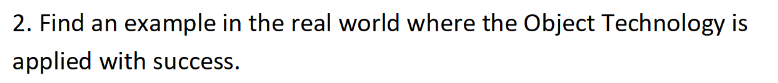
\includegraphics[width=0.8\textwidth]{./Assets/Task requirements/Assignment1/2.png}
    \caption{Problem 2 Task Requirement}
\end{figure}

\begin{itemize}
    \item \textbf{Banking Systems}: Many banking applications use Java for secure, scalable, and maintainable systems, managing accounts, transactions, and user interactions.
    \item \textbf{E-commerce Platforms}: Platforms like eBay and Amazon utilize Java to handle extensive product catalogs, user data, and transactions effectively.
    \item \textbf{Healthcare Systems}: Java is used in healthcare applications for managing patient records, scheduling, and billing, ensuring data integrity and security.
\end{itemize}

\subsection*{Problem 3}

\begin{figure}[H]
    \centering
    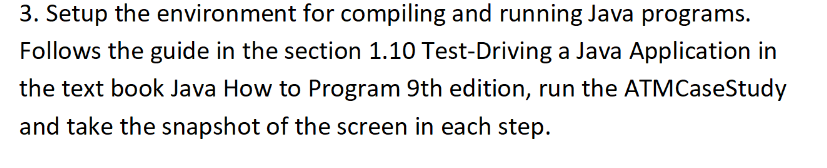
\includegraphics[width=0.8\textwidth]{./Assets/Task requirements/Assignment1/3.png}
    \caption{Problem 3 Task Requirement}
\end{figure}

\begin{figure}[H]
    \centering
    \fbox{\parbox[c][6cm][c]{0.8\textwidth}{\centering Place runtime image here}}
    \caption{Problem 3 Runtime Output}
\end{figure}

\section*{Assignment 2}

\subsection*{2.1 DisplayInitials.java}

\begin{figure}[H]
    \centering
    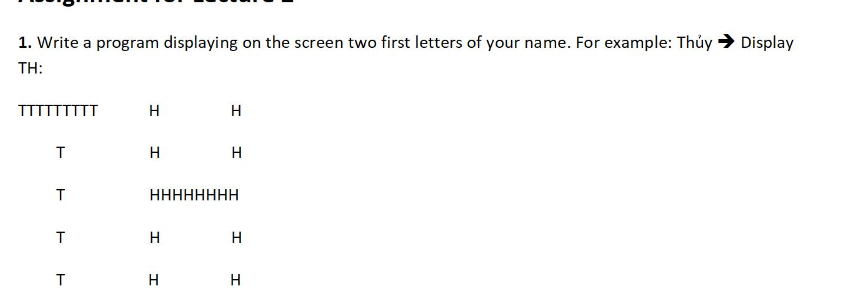
\includegraphics[width=0.8\textwidth]{./Assets/Task requirements/Assignment2/1.png}
    \caption{2.1 Task Requirement}
\end{figure}

\begin{lstlisting}[language=Java, caption=DisplayInitials.java]
import javax.swing.JOptionPane;

public class DisplayIntergers {
    public static void main(String[] args) {
        String firstInput = JOptionPane.showInputDialog("Hay nhap so thu 1:");
        String secondInput = JOptionPane.showInputDialog("Hay nhap so thu 2:");

        int firstNumber = Integer.parseInt(firstInput);
        int secondNumber = Integer.parseInt(secondInput);

        JOptionPane.showMessageDialog(null, "So thu 1: " + firstNumber);
        JOptionPane.showMessageDialog(null, "So thu 2: " + secondNumber);
    }
}
\end{lstlisting}

\subsection*{2.2 (Ex17 - Book) IngredientAdjuster.java}

\begin{figure}[H]
    \centering
    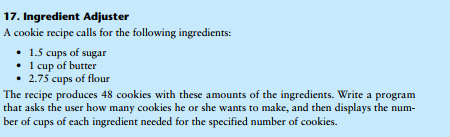
\includegraphics[width=0.8\textwidth]{./Assets/Task requirements/Assignment2/2.17.png}
    \caption{IngredientAdjuster Task Requirement}
\end{figure}

\begin{lstlisting}[language=Java, caption=IngredientAdjuster.java]
import java.util.Scanner;

public class IngredientAdjuster {
    public static void main(String[] args) {
        Scanner scanner = new Scanner(System.in);

        final double sugarPerCookie = 1.5 / 48;
        final double butterPerCookie = 1.0 / 48;
        final double flourPerCookie = 2.75 / 48;

        System.out.print("Enter the number of cookies you want to make: ");
        int cookiesWanted = scanner.nextInt();

        double sugarNeeded = sugarPerCookie * cookiesWanted;
        double butterNeeded = butterPerCookie * cookiesWanted;
        double flourNeeded = flourPerCookie * cookiesWanted;

        System.out.printf("For %d cookies, you need:\n", cookiesWanted);
        System.out.printf("%.2f cups of sugar\n", sugarNeeded);
        System.out.printf("%.2f cups of butter\n", butterNeeded);
        System.out.printf("%.2f cups of flour\n", flourNeeded);

        scanner.close();
    }
}
\end{lstlisting}

\subsection*{(Ex18 - Book) WordGame.java}

\begin{figure}[H]
    \centering
    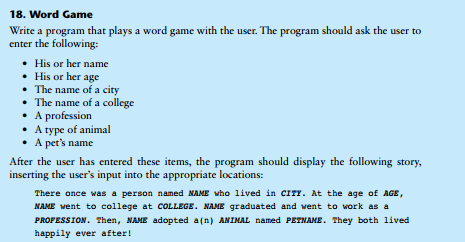
\includegraphics[width=0.8\textwidth]{./Assets/Task requirements/Assignment2/2.18.png}
    \caption{WordGame Task Requirement}
\end{figure}

\begin{lstlisting}[language=Java, caption=WordGame.java]
import java.util.Scanner;

public class WordGame {
    public static void main(String[] args) {
        Scanner scanner = new Scanner(System.in);

        System.out.print("Enter your name: ");
        String name = scanner.nextLine();

        System.out.print("Enter your age: ");
        int age = scanner.nextInt();
        scanner.nextLine();  // Consume the newline

        System.out.print("Enter the name of a city: ");
        String city = scanner.nextLine();

        System.out.print("Enter the name of a college: ");
        String college = scanner.nextLine();

        System.out.print("Enter a profession: ");
        String profession = scanner.nextLine();

        System.out.print("Enter a type of animal: ");
        String animal = scanner.nextLine();

        System.out.print("Enter a pet's name: ");
        String petName = scanner.nextLine();

        System.out.println("\nHere is your story:");
        System.out.println("There once was a person named " + name + " who lived in " + city + ".");
        System.out.println("At the age of " + age + ", " + name + " went to college at " + college + ".");
        System.out.println(name + " graduated and went to work as a(n) " + profession + ".");
        System.out.println("Then, " + name + " adopted a(n) " + animal + " named " + petName + ".");
        System.out.println("They both lived happily ever after!");

        scanner.close();
    }
}
\end{lstlisting}

\subsection*{(Ex19 - Book) StockTransaction.java}


\begin{figure}[H]
    \centering
    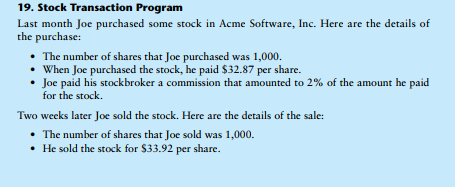
\includegraphics[width=0.8\textwidth]{./Assets/Task requirements/Assignment2/2.19.1.png}
    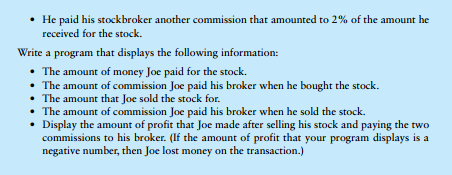
\includegraphics[width=0.8\textwidth]{./Assets/Task requirements/Assignment2/2.19.2.png}
    \caption{StockTransaction Task Requirement}
\end{figure}

\begin{lstlisting}[language=Java, caption=StockTransaction.java]
public class StockTransaction {
    public static void main(String[] args) {
        int sharesBought = 1000;
        double purchasePricePerShare = 32.87;
        double commissionRate = 0.02;
        
        int sharesSold = 1000;
        double salePricePerShare = 33.92;

        double purchaseAmount = sharesBought * purchasePricePerShare;
        double purchaseCommission = purchaseAmount * commissionRate;

        double saleAmount = sharesSold * salePricePerShare;
        double saleCommission = saleAmount * commissionRate;

        double profit = (saleAmount - saleCommission) - (purchaseAmount + purchaseCommission);

        System.out.printf("Amount paid for the stock: $%.2f%n", purchaseAmount);
        System.out.printf("Commission paid on the purchase: $%.2f%n", purchaseCommission);
        System.out.printf("Amount the stock sold for: $%.2f%n", saleAmount);
        System.out.printf("Commission paid on the sale: $%.2f%n", saleCommission);
        System.out.printf("Profit after commissions: $%.2f%n", profit);
    }
}
\end{lstlisting}

\subsection*{2.3 DisplayIntergers.java}

\begin{figure}[H]
    \centering
    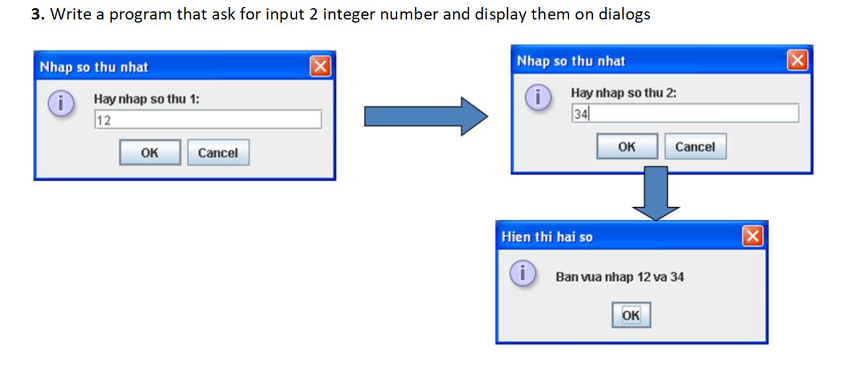
\includegraphics[width=0.8\textwidth]{./Assets/Task requirements/Assignment2/3.png}
    \caption{2.3 Task Requirement}
\end{figure}

\begin{lstlisting}[language=Java, caption=DisplayIntergers.java]
import javax.swing.JOptionPane;

public class DisplayIntergers {
    public static void main(String[] args) {
        String firstInput = JOptionPane.showInputDialog("Hay nhap so thu 1:");
        String secondInput = JOptionPane.showInputDialog("Hay nhap so thu 2:");

        int firstNumber = Integer.parseInt(firstInput);
        int secondNumber = Integer.parseInt(secondInput);

        JOptionPane.showMessageDialog(null, "So thu 1: " + firstNumber);
        JOptionPane.showMessageDialog(null, "So thu 2: " + secondNumber);
    }
}
\end{lstlisting}

\section*{Assignment 3}

\subsection*{1. BMI Measure}
\begin{figure}[H]
    \centering
    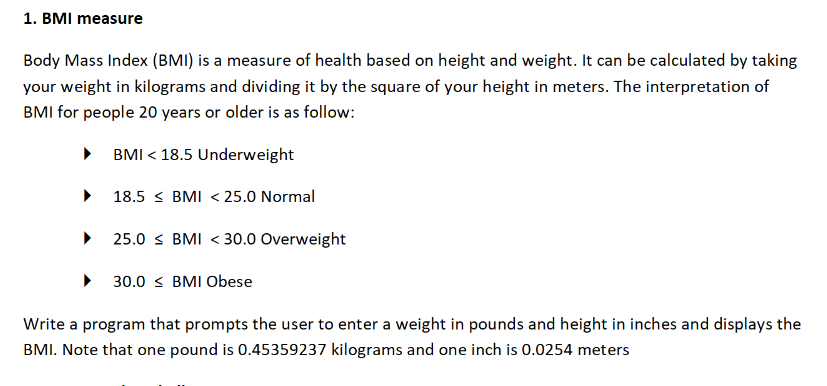
\includegraphics[width=0.8\textwidth]{./Assets/Task requirements/Assignment3/1.png}
    \caption{Problem 1}
\end{figure}

\begin{figure}[h]
    \centering
    \caption{BMI Measure Task Requirement}
\end{figure}

\begin{lstlisting}[language=Java, caption=BMICalculator.java]
import java.util.Scanner;

public class BMICalculator {
    public static void main(String[] args) {
        
        final double POUNDS_TO_KG = 0.45359237;
        final double INCHES_TO_METERS = 0.0254;
        Scanner input = new Scanner(System.in);
        System.out.print("Enter your weight in pounds: ");
        double weightPounds = input.nextDouble();
        System.out.print("Enter your height in inches: ");
        double heightInches = input.nextDouble();
        double weightKg = weightPounds * POUNDS_TO_KG;
        double heightMeters = heightInches * INCHES_TO_METERS;
        double bmi = weightKg / (heightMeters * heightMeters);
        System.out.printf("Your BMI is: %.2f\n", bmi);

        if (bmi < 18.5) {
            System.out.println("Category: Underweight");
        } else if (bmi < 25.0) {
            System.out.println("Category: Normal");
        } else if (bmi < 30.0) {
            System.out.println("Category: Overweight");
        } else {
            System.out.println("Category: Obese");
        }

        input.close();
    }
}
\end{lstlisting}

\subsection*{2. Programming Challenges}

\subsubsection*{3.7 SortedNames.java}
\begin{figure}[H]
    \centering
    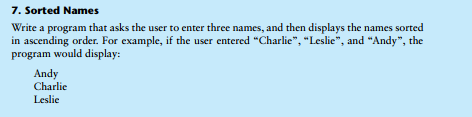
\includegraphics[width=0.8\textwidth]{./Assets/Task requirements/Assignment3/3.7.png}
    \caption{3.7 Task Requirement}
\end{figure}

\begin{figure}[h]
    \centering
    \caption{Programming Challenge 3.7 Task Requirement}
\end{figure}

\begin{lstlisting}[language=Java, caption=SortedNames.java]
import java.util.Arrays;
import java.util.Scanner;

public class SortedNames {
    public static void main(String[] args) {
        Scanner input = new Scanner(System.in);
        System.out.print("Enter the first name: ");
        String name1 = input.nextLine();
        System.out.print("Enter the second name: ");
        String name2 = input.nextLine();
        System.out.print("Enter the third name: ");
        String name3 = input.nextLine();
        String[] names = { name1, name2, name3 };
        Arrays.sort(names);
        System.out.println("\nNames in ascending order:");
        for (String name : names) {
            System.out.println(name);
        }
        input.close();
    }
}
\end{lstlisting}

\subsubsection*{3.8 PackageDiscountCalculator.java}
\begin{figure}[H]
    \centering
    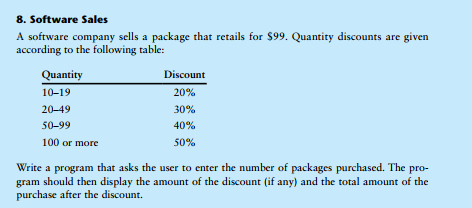
\includegraphics[width=0.8\textwidth]{./Assets/Task requirements/Assignment3/3.8.png}
    \caption{3.8 Task Requirement}
\end{figure}
\begin{figure}[h]
    \centering
    \caption{Programming Challenge 3.8 Task Requirement}
\end{figure}

\begin{lstlisting}[language=Java, caption=PackageDiscountCalculator.java]
import java.util.Scanner;

public class PackageDiscountCalculator {
    public static void main(String[] args) {
        final double PACKAGE_PRICE = 99.0;
        double discountRate = 0;
        Scanner input = new Scanner(System.in);
        System.out.print("Enter the number of packages purchased: ");
        int quantity = input.nextInt();
        if (quantity >= 10 && quantity <= 19) {
            discountRate = 0.20;
        } else if (quantity >= 20 && quantity <= 49) {
            discountRate = 0.30;
        } else if (quantity >= 50 && quantity <= 99) {
            discountRate = 0.40;
        } else if (quantity >= 100) {
            discountRate = 0.50;
        }
        double discountAmount = quantity * PACKAGE_PRICE * discountRate;
        double totalAmount = (quantity * PACKAGE_PRICE) - discountAmount;
        System.out.println("Discount amount: $" + discountAmount);
        System.out.println("Total amount after discount: $" + totalAmount);
        input.close();
    }
}
\end{lstlisting}

\subsubsection*{3.9 ShippingCharges.java}
\begin{figure}[H]
    \centering
    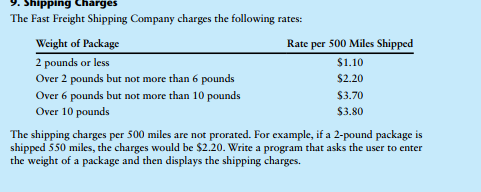
\includegraphics[width=0.8\textwidth]{./Assets/Task requirements/Assignment3/3.9.png}
    \caption{ 3.9 Task Requirement}
\end{figure}
\begin{figure}[h]
    \centering
    \caption{Programming Challenge 3.9 Task Requirement}
\end{figure}

\begin{lstlisting}[language=Java, caption=ShippingCharges.java]
import java.util.Scanner;

public class ShippingCharges {
    public static void main(String[] args) {
        final double RATE_2_POUNDS = 1.10;
        final double RATE_2_TO_6_POUNDS = 2.20;
        final double RATE_6_TO_10_POUNDS = 3.70;
        final double RATE_10_POUNDS = 3.80;
        Scanner input = new Scanner(System.in);
        System.out.print("Enter the weight of the package (in pounds): ");
        double weight = input.nextDouble();
        System.out.print("Enter the distance to be shipped (in miles): ");
        int distance = input.nextInt();
        int increments = (int) Math.ceil(distance / 500.0);
        double rate;
        if (weight <= 2) {
            rate = RATE_2_POUNDS;
        } else if (weight <= 6) {
            rate = RATE_2_TO_6_POUNDS;
        } else if (weight <= 10) {
            rate = RATE_6_TO_10_POUNDS;
        } else {
            rate = RATE_10_POUNDS;
        }
        double totalCharges = rate * increments;
        System.out.printf("The shipping charges are: $%.2f\n", totalCharges);
        input.close();
    }
}
\end{lstlisting}

\section*{Assignment 5}

\subsection*{1. Occurrence of max numbers}
\begin{figure}[H]
    \centering
    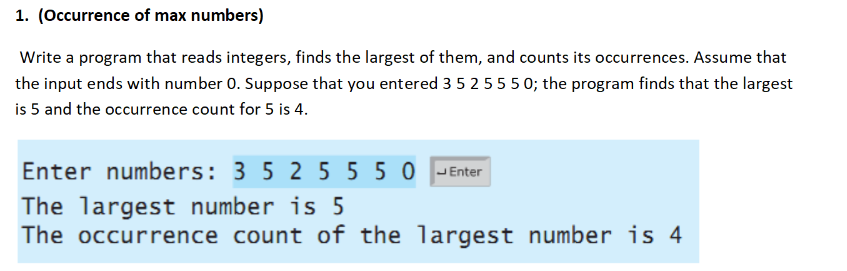
\includegraphics[width=0.8\textwidth]{./Assets/Task requirements/Assignment5/1.png}
    \caption{Problem 1 Task Requirement}
\end{figure}

\begin{figure}[h]
    \centering
    \caption{Task Requirement}
\end{figure}

\begin{lstlisting}[language=Java, caption=MaxNumCounter.java]
package OccurenceOfMaxNum;

import java.util.Scanner;

public class MaxNumCounter {
    public static void main(String[] args) {
        Scanner scanner = new Scanner(System.in);
        System.out.println("(The program will read integers input til the first 0)");
        System.out.println("Enter numbers:");
        findLargestAndCount(scanner);
        scanner.close();
    }

    public static void findLargestAndCount(Scanner scanner) {
        int max = 0;
        int count = 1;

        while (true) {
            if (scanner.hasNextInt()) {
                int number = scanner.nextInt();
                if (number == 0) {
                    break;
                }
                if (number > max) {
                    max = number;
                    count = 1;
                } else if (number == max) {
                    count++;
                }
            } else {
                System.out.println("Invalid input (not integers) ignored.");
                scanner.next(); // Clear the invalid input
            }
        }

        if (max != 0) {
            System.out.println("The largest number is " + max);
            System.out.println("The occurrence count of the largest number is " + count);
        } else {
            System.out.println("The largest number is 0");
            System.out.println("The occurrence count of the largest number is 1");
        }
    }
}
\end{lstlisting}

\subsection*{2. Programming Challenges}

\subsubsection*{Challenge 1}
\begin{figure}[H]
    \centering
    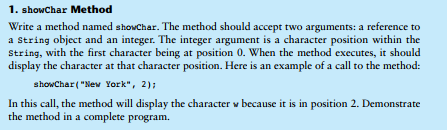
\includegraphics[width=0.8\textwidth]{./Assets/Task requirements/Assignment5/5.1.png}
    \caption{5.1 Task Requirement}
\end{figure}
\begin{figure}[h]
    \centering
    \caption{Task Requirement}
\end{figure}

\begin{lstlisting}[language=Java, caption=Challenge1.java]
package ProgrammingChallenges;
import java.util.Scanner;

public class challenge1 {
    public static void main(String[] args) {

        Scanner scanner = new Scanner(System.in);

        //Input string
        System.out.print("Enter a string: ");
        String inputString = scanner.nextLine();

        //Input position
        int position;
        while (true) {
            System.out.print("Enter a position: ");
            position = scanner.nextInt();

            // Check if the position is valid
            if (position >= 0 && position < inputString.length()) {
                break;
            } else {
                System.out.println("Invalid position. Please enter a position between 0 and " + (inputString.length() - 1));
            }
        }

        // Call the showChar method with the user inputs
        showChar(inputString, position);

        scanner.close();
    }

    public static void showChar(String str, int position) {
        if (position >= 0 && position < str.length()) {
            char ch = str.charAt(position);
            System.out.println("The character at position " + position + " is " + ch);
        } else {
            System.out.println("Invalid position. Please enter a position between 0 and " + (str.length() - 1));
        }
    }
}
\end{lstlisting}

\subsubsection*{Challlenge 2}
\begin{figure}[H]
    \centering
    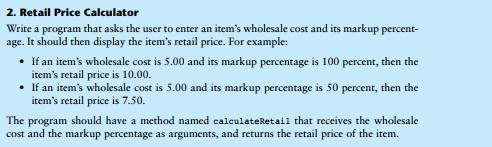
\includegraphics[width=0.8\textwidth]{./Assets/Task requirements/Assignment5/5.2.png}
    \caption{5.2 Task Requirement}
\end{figure}

\begin{figure}[h]
    \centering
    \caption{Task Requirement}
\end{figure}

\begin{lstlisting}[language=Java, caption=Challenge2.java]
package ProgrammingChallenges;

import java.util.Scanner;

public class challenge2 {
    public static void main(String[] args) {
        Scanner scanner = new Scanner(System.in);

        // Input the wholesale cost
        System.out.print("Enter the item's wholesale cost: ");
        double wholesaleCost = scanner.nextDouble();

        //Input the markup percentage
        System.out.print("Enter the item's markup percentage: ");
        double markupPercentage = scanner.nextDouble();

        // Calculate the retail price
        double retailPrice = calculateRetail(wholesaleCost, markupPercentage);

        // Display the retail price
        System.out.printf("The item's retail price is: %.2f%n", retailPrice);

        scanner.close();
    }

    public static double calculateRetail(double wholesaleCost, double markupPercentage) {
        return wholesaleCost + (wholesaleCost * markupPercentage / 100);
    }
}
\end{lstlisting}

\subsubsection*{Challenge 4}
\begin{figure}[H]
    \centering
    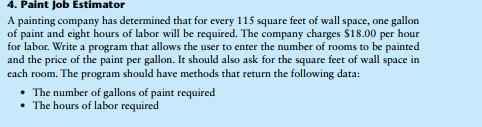
\includegraphics[width=0.8\textwidth]{./Assets/Task requirements/Assignment5/5.4.1.png}
    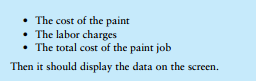
\includegraphics[width=0.8\textwidth]{./Assets/Task requirements/Assignment5/5.4.2.png}
    \caption{5.4 Task Requirement}
\end{figure}

\begin{figure}[h]
    \centering
    \caption{Task Requirement}
\end{figure}

\begin{lstlisting}[language=Java, caption=Challenge4.java]
package ProgrammingChallenges;

import java.util.Scanner;

public class challenge4 {
    public static void main(String[] args) {
        Scanner scanner = new Scanner(System.in);

        // Input the number of rooms
        int numberOfRooms = getValidIntInput(scanner, "Enter the number of rooms to be painted: ");

        // Input the price of the paint per gallon
        double pricePerGallon = getValidDoubleInput(scanner, "Enter the price of the paint per gallon: ");

        // Initialize total square feet
        double totalSquareFeet = 0;

        // Input the square feet of wall space for each room
        for (int i = 1; i <= numberOfRooms; i++) {
            totalSquareFeet += getValidDoubleInput(scanner, "Enter the square feet of wall space for room " + i + ": ");
        }

        // Calculate the required data
        double gallonsOfPaintRequired = calculateGallonsOfPaintRequired(totalSquareFeet);
        double hoursOfLaborRequired = calculateHoursOfLaborRequired(totalSquareFeet);
        double costOfPaint = calculateCostOfPaint(gallonsOfPaintRequired, pricePerGallon);
        double laborCharges = calculateLaborCharges(hoursOfLaborRequired);
        double totalCost = calculateTotalCost(costOfPaint, laborCharges);

        // Display the results
        System.out.printf("The numbers of gallons of paint required: %.2f%n", gallonsOfPaintRequired);
        System.out.printf("The hours of labor required: %.2f%n", hoursOfLaborRequired);
        System.out.printf("The cost of the paint: $%.2f%n", costOfPaint);
        System.out.printf("The labor charges: $%.2f%n", laborCharges);
        System.out.printf("The total cost of the paint job: $%.2f%n", totalCost);

        scanner.close();
    }

    public static int getValidIntInput(Scanner scanner, String prompt) {
        int input;
        while (true) {
            System.out.print(prompt);
            if (scanner.hasNextInt()) {
                input = scanner.nextInt();
                scanner.nextLine(); // Consume the newline character
                break;
            } else {
                System.out.println("Invalid input. Please enter a valid integer.");
                scanner.next(); // Clear the invalid input
            }
        }
        return input;
    }

    public static double getValidDoubleInput(Scanner scanner, String prompt) {
        double input;
        while (true) {
            System.out.print(prompt);
            if (scanner.hasNextDouble()) {
                input = scanner.nextDouble();
                scanner.nextLine(); // Consume the newline character
                break;
            } else {
                System.out.println("Invalid input. Please enter a valid number.");
                scanner.next(); // Clear the invalid input
            }
        }
        return input;
    }

    public static double calculateGallonsOfPaintRequired(double totalSquareFeet) {
        return totalSquareFeet / 115;
    }

    public static double calculateHoursOfLaborRequired(double totalSquareFeet) {
        return (totalSquareFeet / 115) * 8;
    }

    public static double calculateCostOfPaint(double gallonsOfPaintRequired, double pricePerGallon) {
        return gallonsOfPaintRequired * pricePerGallon;
    }

    public static double calculateLaborCharges(double hoursOfLaborRequired) {
        return hoursOfLaborRequired * 18.00;
    }

    public static double calculateTotalCost(double costOfPaint, double laborCharges) {
        return costOfPaint + laborCharges;
    }
}
\end{lstlisting}

\subsection*{3. Multiplication Table}
\begin{figure}[H]
    \centering
    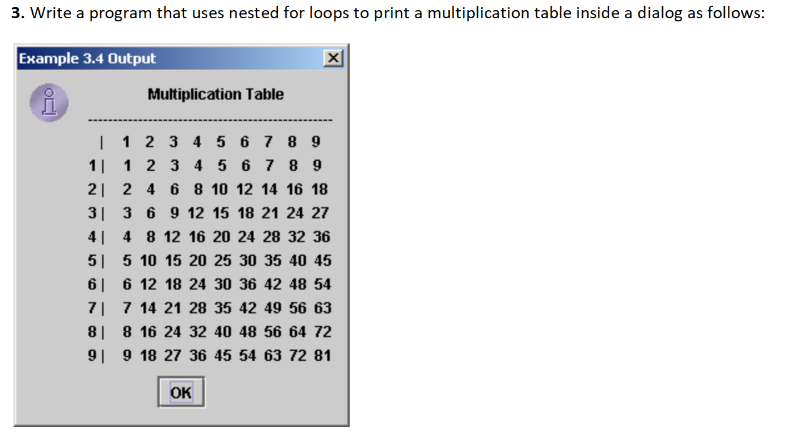
\includegraphics[width=0.8\textwidth]{./Assets/Task requirements/Assignment5/3.png}
    
    \caption{Problem 3 Task Requirement}
\end{figure}

\begin{figure}[h]
    \centering
    \caption{Task Requirement}
\end{figure}

\begin{lstlisting}[language=Java, caption=MultiplicationTable.java]
package MultiplicationTable;

import javax.swing.JOptionPane;

public class MultiplicationTable {
    public static void main(String[] args) {
        StringBuilder table = new StringBuilder();

        // Add the header and underline
        table.append("Multiplication Table\n");
        table.append("-------------------------------------------------------\n");

        // Add the top row of numbers
        table.append("    |");
        for (int i = 1; i <= 9; i++) {
            table.append(String.format("%6d", i));
        }
        table.append("\n");

        // Create the multiplication table using nested for loops
        for (int i = 1; i <= 9; i++) {
            table.append(String.format("%2d |", i));
            for (int j = 1; j <= 9; j++) {
                if (i*j >= 10){
                table.append(String.format("%5d", i * j));
                } else table.append(String.format("%6d", i * j));
            }
            table.append("\n");
        }

        // Display the multiplication table in a dialog box with the specified header
        JOptionPane.showMessageDialog(null, table.toString(), "Example 3.4 Output", JOptionPane.INFORMATION_MESSAGE);
    }
}
\end{lstlisting}

% Begin Assignment 6
\section*{Assignment 6}

\subsection*{1. Implementation of Student Class}
\begin{figure}[H]
    \centering
    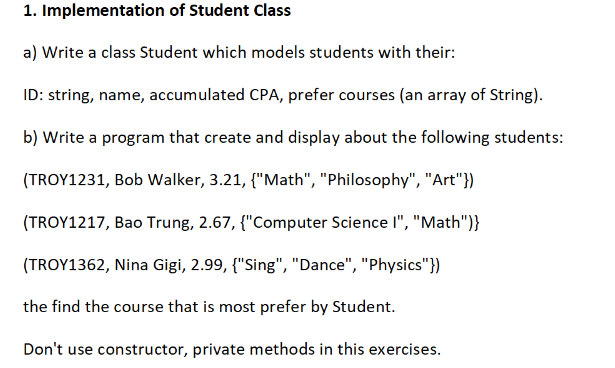
\includegraphics[width=0.8\textwidth]{./Assets/Task requirements/Assignment6/1.png}
    
    \caption{Problem 1 Task Requirement}
\end{figure}

% Placeholder for Task Requirement Image
\begin{figure}[h]
    \centering
    % Replace 'path/to/student_task_requirement.png' with the actual path to your image
    \caption{Student Class Task Requirement}
\end{figure}

% Insert Student.java code here
\begin{lstlisting}[language=Java, caption=Student.java]
import java.util.Arrays;

public class Student {
    private String id;
    private String name;
    private double accumulatedCPA;
    private String[] preferCourse;

    public String getId() {
        return id;
    }

    public void setId(String id) {
        this.id = id;
    }

    public String getName() {
        return name;
    }

    public void setName(String name) {
        this.name = name;
    }

    public double getAccumulatedCPA() {
        return accumulatedCPA;
    }

    public void setAccumulatedCPA(double accumulatedCPA) {
        this.accumulatedCPA = accumulatedCPA;
    }

    public String[] getPreferCourse() {
        return preferCourse;
    }

    public void setPreferCourse(String[] preferCourse) {
        this.preferCourse = preferCourse;
    }

    public String studentGetInfo(){
        return this.getId() + " | Student name: " + this.getName() + " | Accumulated CPA:  " + this.getAccumulatedCPA() + " | Student prefer course: " + Arrays.toString(this.getPreferCourse());
    }
}
\end{lstlisting}

% Insert Main.java code here
\begin{lstlisting}[language=Java, caption=Main.java]
public class Main {
    public static void main(String[] args) {
        Student Bob = new Student();
        Bob.setId("TROY1231");
        Bob.setName("Bob Walker");
        Bob.setAccumulatedCPA(3.21);
        Bob.setPreferCourse(new String[] {"Math", "Philosophy", "Art"});

        Student Trung = new Student();
        Trung.setId("TROY1217");
        Trung.setName("Bao Trung");
        Trung.setAccumulatedCPA(2.67);
        Trung.setPreferCourse(new String[] {"Computer Science I", "Math"});

        Student Nina = new Student();
        Nina.setId("TROY1362");
        Nina.setName("Nina Gigi");
        Nina.setAccumulatedCPA(2.99);
        Nina.setPreferCourse(new String[] {"Sing", "Dance", "Physics"});

        System.out.println(Bob.studentGetInfo());
        System.out.println(Trung.studentGetInfo());
        System.out.println(Nina.studentGetInfo());
    }
}
\end{lstlisting}

\subsection*{2. Implementation of TV Class}
\begin{figure}[H]
    \centering
    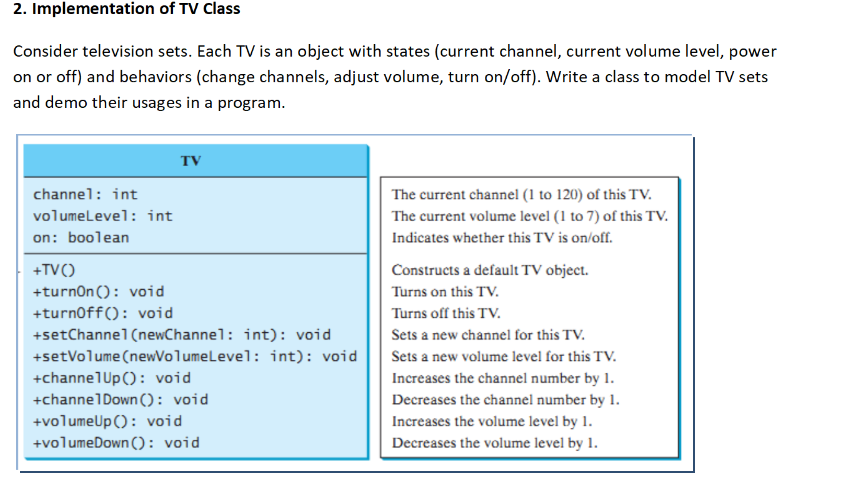
\includegraphics[width=0.8\textwidth]{./Assets/Task requirements/Assignment6/2.png}
    
    \caption{Problem 2 Task Requirement}
\end{figure}

% Placeholder for Task Requirement Image
\begin{figure}[h]
    \centering
    % Replace 'path/to/tv_task_requirement.png' with the actual path to your image
    \caption{TV Class Task Requirement}
\end{figure}

% Insert TV.java code here
\begin{lstlisting}[language=Java, caption=TV.java]
public class TV {
    private int channel;
    private int volumeLevel;
    private boolean on;

        private static final int MAX_CHANNEL = 1000;
    private static final int MIN_CHANNEL = 0;
    private static final int MAX_VOLUME = 100;
    private static final int MIN_VOLUME = 0;

    TV() {
        this.channel = MIN_CHANNEL;
        this.volumeLevel = 50;
        this.on = false;
    }

    public void turnOn() {
        this.on = true;
        System.out.println("TV turned on");
    }

    public void turnOff() {
        System.out.println("TV turning off");
        this.on = false;
    }

    private void currentVolume() {
        System.out.println("Current volume: " + this.volumeLevel);
    }

    private void currentChannel() {
        System.out.println("Channel: " + this.channel);
    }

    public void setChannel(int newChannel) {
        if(this.on && newChannel >= MIN_CHANNEL && newChannel <= MAX_CHANNEL) {
            this.channel = newChannel;
            currentChannel();
        }
    }

    public void setVolume(int newVolumeLevel) {
        if(this.on && newVolumeLevel >= MIN_VOLUME && newVolumeLevel <= MAX_VOLUME && newVolumeLevel % 5 == 0) {
            this.volumeLevel = newVolumeLevel;
            currentVolume();
        }
    }

    public void channelUp() {
        if(this.on && this.channel + 1 <= MAX_CHANNEL) {
            this.channel++;
            currentChannel();
        }
    }

    public void channelDown() {
        if(this.on && this.channel - 1 >= MIN_CHANNEL) {
                this.channel--;
                currentChannel();
        }
    }

    public void volumeUp() {
        if(this.on && volumeLevel + 5 <= MAX_VOLUME) {
                this.volumeLevel += 5;
                currentVolume();
        }
    }

    public void volumeDown() {
        if (this.on && volumeLevel - 5 >= MIN_VOLUME) {
                this.volumeLevel -= 5;
                currentVolume();
        }
    }
}
\end{lstlisting}

% Insert Main.java code here
\begin{lstlisting}[language=Java, caption=Main.java]

public class Main {
    public static void main(String[] args) {
        TV SamsungTV = new TV();
        SamsungTV.setChannel(45);
        SamsungTV.setVolume(25);
        SamsungTV.volumeUp();

        SamsungTV.turnOn();
        SamsungTV.setVolume(25);
        SamsungTV.volumeUp();
        SamsungTV.volumeDown();
        SamsungTV.channelDown();
        SamsungTV.channelUp();
        SamsungTV.setChannel(123);
        SamsungTV.setChannel(1230);
        SamsungTV.turnOff();
    }
}
\end{lstlisting}

\subsection*{6.1 Employee Class}
\begin{figure}[H]
    \centering
    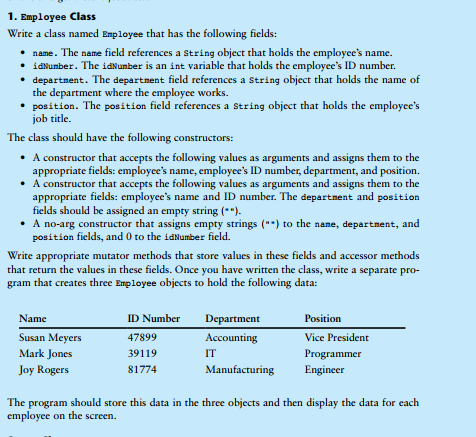
\includegraphics[width=0.8\textwidth]{./Assets/Task requirements/Assignment6/6.1.png}
    
    \caption{6.1Task Requirement}
\end{figure}

% Placeholder for Task Requirement Image
\begin{figure}[h]
    \centering
    % Replace 'path/to/employee_task_requirement.png' with the actual path to your image
    \caption{Employee Class Task Requirement}
\end{figure}

% Insert Employee.java code here
\begin{lstlisting}[language=Java, caption=Employee.java]
package employeeClass;

public class Employee {
    private String name;
    private int idNumber;
    private String department;
    private String position;

    public Employee(String name, int idNumber, String department, String position) {
        this.name = name;
        this.idNumber = idNumber;
        this.department = department;
        this.position = position;
    }

    public Employee(String name, int idNumber) {
        this(name, idNumber, "", "");
    }

    public Employee() {
        this("", 0, "", "");
    }

    public void setName(String name) {
        this.name = name;
    }

    public void setIdNumber(int idNumber) {
        this.idNumber = idNumber;
    }

    public void setDepartment(String department) {
        this.department = department;
    }

    public void setPosition(String position) {
        this.position = position;
    }

    public String getName() {
        return name;
    }

    public int getIdNumber() {
        return idNumber;
    }

    public String getDepartment() {
        return department;
    }

    public String getPosition() {
        return position;
    }
}

\end{lstlisting}

% Insert Main.java code here
\begin{lstlisting}[language=Java, caption=Main.java]
package employeeClass;


public class Main {
    public static void main(String[] args) {
                Employee employee1 = new Employee("Susan Meyers", 47899, "Accounting", "Vice President");
                Employee employee2 = new Employee("Mark Jones", 39119, "IT", "Programmer");
                Employee employee3 = new Employee("Joy Rogers", 81774, "Manufacturing", "Engineer");

                displayEmployeeInfo(employee1);
                displayEmployeeInfo(employee2);
                displayEmployeeInfo(employee3);
            }

            public static void displayEmployeeInfo(Employee employee) {
                System.out.printf(" Name: "    + employee.getName());
                System.out.printf(" | ID Number: " + employee.getIdNumber());
                System.out.printf(" | Department: " + employee.getDepartment());
                System.out.printf(" | Position: " + employee.getPosition());
                System.out.println();
        }
    }
\end{lstlisting}

\subsection*{6.2 Car Class}
\begin{figure}[H]
    \centering
    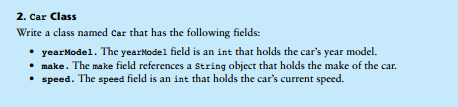
\includegraphics[width=0.8\textwidth]{./Assets/Task requirements/Assignment6/6.2.1.png}
    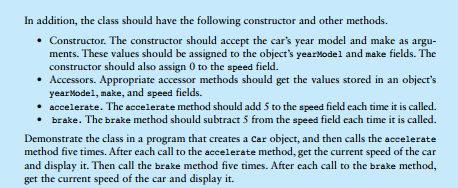
\includegraphics[width=0.8\textwidth]{./Assets/Task requirements/Assignment6/6.2.2.png}
    \caption{6.2 Task Requirement}
\end{figure}

% Placeholder for Task Requirement Image
\begin{figure}[h]
    \centering
    % Replace 'path/to/car_task_requirement.png' with the actual path to your image
    \caption{Car Class Task Requirement}
\end{figure}

% Insert Car.java code here
\begin{lstlisting}[language=Java, caption=Car.java]
package carClass;

public class Car {
    private int yearModel;
    private String make;
    private int speed;

    public Car(int yearModel, String make) {
        this.yearModel = yearModel;
        this.make = make;
        this.speed = 0;
    }

    public int getYearModel() {
        return yearModel;
    }

    public String getMake() {
        return make;
    }

    public int getSpeed() {
        return speed;
    }

    public void accelerate() {
        speed += 10;
    }

    public void brake() {
        if (speed >= 10) {
            speed -= 10;
        } else {
            speed = 0;
        }
    }
}

\end{lstlisting}

% Insert Main.java code here
\begin{lstlisting}[language=Java, caption=Main.java]
package carClass;

public class Main {
    public static void main(String[] args) {
        // Create a Car object
        Car car = new Car(2023, "Toyota");

        // Accelerate the car five times and display the speed after each acceleration
        System.out.println("Accelerating...");
        for (int i = 1; i <= 5; i++) {
            car.accelerate();
            System.out.println("Current speed after acceleration " + i + ": " + car.getSpeed() + " mph");
        }

        // Brake the car five times and display the speed after each brake
        System.out.println("\nBraking...");
        for (int i = 1; i <= 5; i++) {
            car.brake();
            System.out.println("Current speed after brake " + i + ": " + car.getSpeed() + " mph");
        }
    }

}

\end{lstlisting}

\subsection*{6.3 Person Information Class}
\begin{figure}[H]
    \centering
    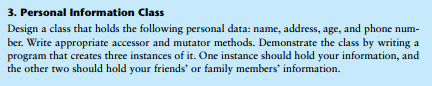
\includegraphics[width=0.8\textwidth]{./Assets/Task requirements/Assignment6/6.3.png}
    
    \caption{6.3 Task Requirement}
\end{figure}

% Placeholder for Task Requirement Image
\begin{figure}[h]
    \centering
    % Replace 'path/to/person_task_requirement.png' with the actual path to your image
    \caption{Person Information Class Task Requirement}
\end{figure}

% Insert Person.java code here
\begin{lstlisting}[language=Java, caption=Person.java]
package personInformationClass;

public class Person {
    private String name;
    private String address;
    private int age;
    private String phoneNumber;

    public Person(String name, String address, int age, String phoneNumber) {
        this.name = name;
        this.address = address;
        this.age = age;
        this.phoneNumber = phoneNumber;
    }

    public String getName() {
        return name;
    }

    public String getAddress() {
        return address;
    }

    public int getAge() {
        return age;
    }

    public String getPhoneNumber() {
        return phoneNumber;
    }

    public void setName(String name) {
        this.name = name;
    }

    public void setAddress(String address) {
        this.address = address;
    }

    public void setAge(int age) {
        this.age = age;
    }

    public void setPhoneNumber(String phoneNumber) {
        this.phoneNumber = phoneNumber;
    }
}

\end{lstlisting}

% Insert Main.java code here
\begin{lstlisting}[language=Java, caption=Main.java]
package personInformationClass;

public class Main {
    public static void main(String[] args) {
        Person myInfo = new Person("Your Name", "123 Main St, Hometown", 30, "555-1234");
        Person friendInfo = new Person("Friend Name", "456 Maple Ave, Nearby Town", 25, "555-5678");
        Person familyMemberInfo = new Person("Family Member Name", "789 Oak Dr, Family Town", 55, "555-8765");

        displayPersonInfo(myInfo);
        displayPersonInfo(friendInfo);
        displayPersonInfo(familyMemberInfo);
    }

    public static void displayPersonInfo(Person person) {
        System.out.println("Name: " + person.getName());
        System.out.println("Address: " + person.getAddress());
        System.out.println("Age: " + person.getAge());
        System.out.println("Phone Number: " + person.getPhoneNumber());
        System.out.println();
    }
}

\end{lstlisting}

\subsection*{6.4 RetailItem Class}
\begin{figure}[H]
    \centering
    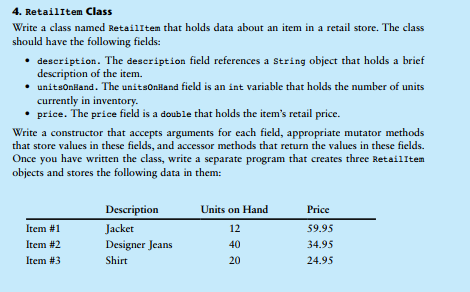
\includegraphics[width=0.8\textwidth]{./Assets/Task requirements/Assignment6/6.4.png}
   
    \caption{6.4 Task Requirement}
\end{figure}

% Placeholder for Task Requirement Image
\begin{figure}[h]
    \centering
    % Replace 'path/to/retailitem_task_requirement.png' with the actual path to your image
    \caption{RetailItem Class Task Requirement}
\end{figure}

% Insert RetailItem.java code here
\begin{lstlisting}[language=Java, caption=RetailItem.java]
package retailItem;

public class RetailItem {
    private String description;
    private int unitsOnHand;
    private double price;

    public RetailItem(String description, int unitsOnHand, double price) {
        this.description = description;
        this.unitsOnHand = unitsOnHand;
        this.price = price;
    }

    public String getDescription() {
        return description;
    }

    public int getUnitsOnHand() {
        return unitsOnHand;
    }

    public double getPrice() {
        return price;
    }

    public void setDescription(String description) {
        this.description = description;
    }

    public void setUnitsOnHand(int unitsOnHand) {
        this.unitsOnHand = unitsOnHand;
    }

    public void setPrice(double price) {
        this.price = price;
    }
}

\end{lstlisting}

% Insert Main.java code here
\begin{lstlisting}[language=Java, caption=Main.java]
package retailItem;

public class Main {
        public static void main(String[] args) {
            RetailItem item1 = new RetailItem("Jacket", 12, 59.95);
            RetailItem item2 = new RetailItem("Designer Jeans", 40, 34.95);
            RetailItem item3 = new RetailItem("Shirt", 20, 24.95);

            displayItemInfo(item1);
            displayItemInfo(item2);
            displayItemInfo(item3);
        }

        public static void displayItemInfo(RetailItem item) {
            System.out.println("Description: " + item.getDescription());
            System.out.println("Units on Hand: " + item.getUnitsOnHand());
            System.out.println("Price: $" + item.getPrice());
            System.out.println();
        }

}

\end{lstlisting}

% End of Assignment 6

\end{document}